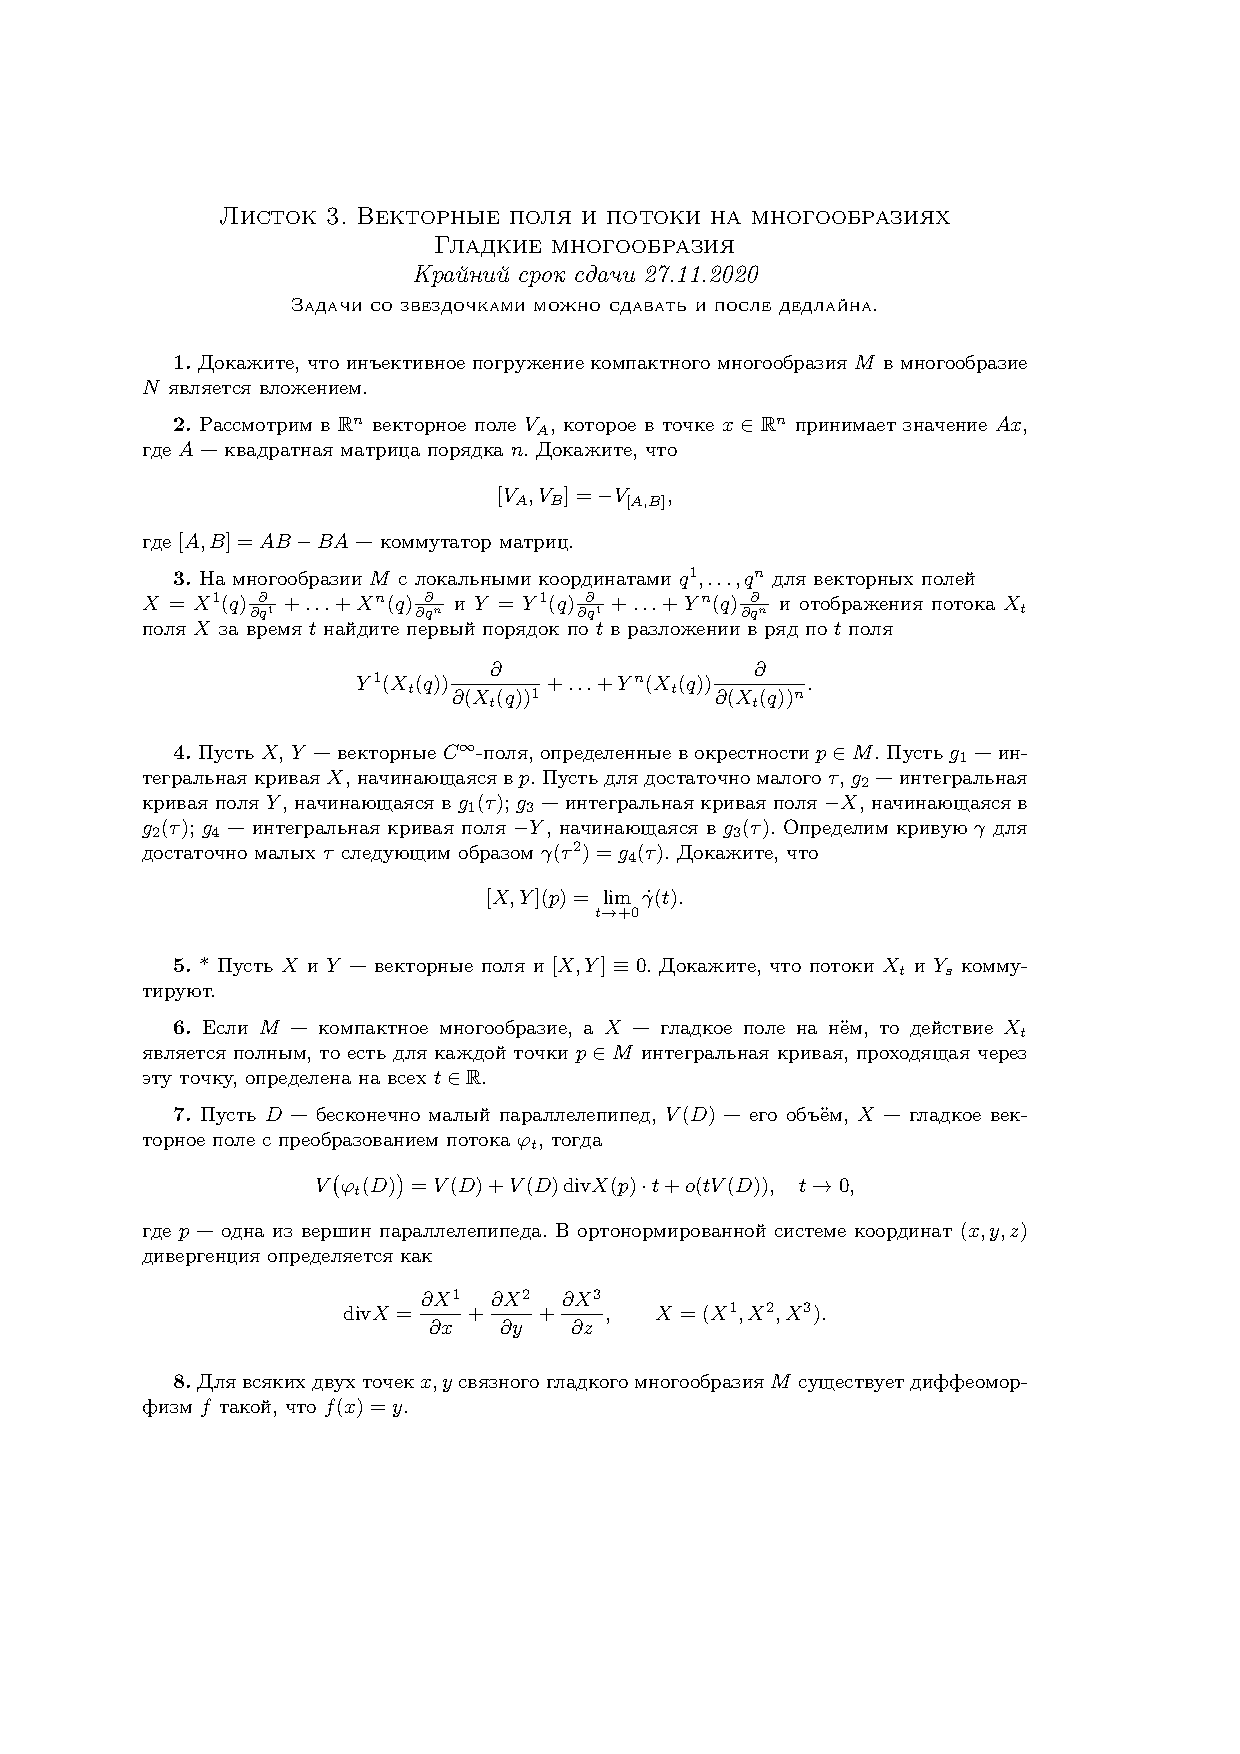
\includepdf[scale=0.95,pages=1,pagecommand=\section*{Условия}]{Tasks/Probl-manif3}
\newpage
\section*{Решения}
\subsection*{Задача 1}
	Заметим, что факт того, что $F$ -- гомеоморфизм на образ равносилен тому, что $F$ -- непрерывная биекция на образ, $F^{-1}$ непрерывна.\\
	$F$ -- гладкая, следовательно непрерывная. $N$ -- многообразие, следовательно оно хаусдорфово и $F$ -- непрерывное отображение из компактного многообразие в хаусдорфово. Тогда из курса топологии известно, что $F$ -- замкнута (и прообраз замкнутого замкнут), Тогда $F^{-1}$ непрерывна ($A \subset M$ -- компакт, то $F(A)$ -- компакт в хаусдорфовом, а следовательно $F(A)$ замкнуто). Тогда так как $F$ -- инъекция, то $F$ -- биекция на образ (то есть $M$ и $F(M)$ биективны), откуда следует, что $F$ -- гомеоморфизм на образ, а следовательно вложение.
\vskip0.5in
	
	
\subsection*{Задача 2}
	Распишем векторные поля по определению
	\begin{gather*}
		V_A := \sum\limits_i a_i(x) \frac{\partial }{\partial x^{i}}\qquad a_j(x) = \sum\limits_{m} A_{jm}x_m\\
		V_B := \sum\limits_i b_i(x) \frac{\partial }{\partial x^{i}}\qquad b_j(x) = \sum\limits_{m} B_{jm}x_m\\
		\sum\limits_{i} \frac{\partial b_j}{\partial x_i} = 
		\sum\limits_{i} \left( \frac{\partial  \sum\limits_{m} B_{jm} x_m}{\partial x_i}\right) =
		\sum\limits_{i} B_{ij}\\
		\frac{\partial a_j}{\partial x_i} = \sum\limits_{i} A_{ij}
	\end{gather*}
	Распишем коммутатор векторных полей
	\begin{gather*}
		[V_A,V_B] = 
		\sum\limits_{i}(a_i(x)B_{ij} - b_i(x) A_{ji}) = 
		\sum\limits_{i}\left(\left(\sum\limits_{m} A_{im}x_m\right)B_{ji} - \left(\sum\limits_{m} B_{im}x_m\right)A_{ji}\right) =\\
		\sum\limits_{i} \sum\limits_{m} \left(A_{im} B_{ji} - B_{im} A_{ji}\right) x_m =
		\sum\limits_{m} \sum\limits_{i} \left(B_{ji} A_{im} - A_{ji} B_{im}\right) x_m
	\end{gather*}
	Последний переход можно сделать так как
	\begin{gather*}
		\sum\limits_{i} \sum\limits_{m} A_{im} B_{ji} = 
		\sum\limits_{i} (A_{i1} B_{ji} + A_{i2} B_{ji} + \ldots + A_{in} B_{ji}) =
		\sum\limits_{i} (B_{ji} A_{i1} + B_{ji} A_{i2} + \ldots + B_{ji} A_{in}) =
		\sum\limits_{m} \sum\limits_{i} B_{ji} A_{im}
	\end{gather*} 
	Тогда
	\begin{gather*}
		-V_{[A,B]} = V_{[B,A]} = V_{BA - AB} =
		\sum\limits_{i} c_i(x) \frac{\partial }{\partial x^{i}} =
		\sum\limits_{m} c_{im} x_{m} =
		\sum\limits_{m} \left(\sum\limits_{i} (B_{ji} A_{im} - A_{ji} B_{im}) x_m \right)
	\end{gather*}
\vskip0.5in

\begin{comment}
	По определению
\begin{gather*}
V_A(x)(f) := A_{ij}x_{j}\frac{\partial f}{\partial x_i}\\
V_B(x)(f) := B_{ij}x_{j}\frac{\partial f}{\partial x_i}
\end{gather*}
Тогда распишем $[V_A,V_B]$
\begin{gather*}
(V_A(x) \circ V_B(x))(f) := V_A(x)(V_B(x)(f)) = 
A_{ij}B_{ki}x_j \frac{\partial f}{\partial x_k} + A_{ij}B_{kl}x_j x_l \frac{\partial^2 f}{\partial x_i x_k}\\
(V_B(x) \circ V_A(x))(f) := V_B(x)(V_A(x)(f)) = 
B_{kl}A_{ik}x_l \frac{\partial f}{\partial x_i} + B_{kl}A_{ij}x_l x_j \frac{\partial^2 f}{\partial x_k x_i}\\
V_A(x)(V_B(x)(f)) - V_B(x)(V_A(x)(f)) = 
\left(A_{ij}B_{ki}x_j \frac{\partial f}{\partial x_k} + A_{ij}B_{kl}x_j x_l \frac{\partial^2 f}{\partial x_i x_k}\right) - 
\left(B_{kl}A_{ik}x_l \frac{\partial f}{\partial x_i} + B_{kl}A_{ij}x_l x_j \frac{\partial^2 f}{\partial x_k x_i}\right)
\end{gather*}
И распишем $V_{[A,B]}$
\begin{gather*}
V_{[A,B]}(x)(f) := [A,B]_{kj} x_{j} \frac{\partial f}{\partial x_k} = (A_{ki}B_{ij} - B_{ki}A_{ij})x_j \frac{\partial f}{\partial x_k}
\end{gather*}
Откуда
\begin{gather*}
[V_A(x),V_B(x)] = -V_{[A,B]}(x)
\end{gather*}
\end{comment}


\subsection*{Задача 3}
	Введем $\gamma_q(0) = q$ такое что $\frac{\partial \gamma_q(r)}{\partial r}|_{r = 0} = X_q$
	Разложим в ряд тейлора по $t$
	\begin{gather*}
		X_t(q) = \gamma_q(t) = q + tX_q + o(t)\\
		Y^{i}(X_t(q)) = Y^{i}(q + tX_q + o(t))\\
		\frac{\partial Y^{i}(X_t(q))}{\partial t}|_{t = 0} = \sum\limits_{j = 0}^{n} \frac{\partial Y^{i}}{\partial q^{j}} x^{j}(q)\\
		Y^{i}(X_t(q)) = Y^{i}(q) + t\left(\sum\limits_{j = 0}^{n} \frac{\partial Y^{i}}{\partial q^{j}} X^{i}(q)\right) + o(t)\\
		\frac{\partial }{\partial (X_t(q))^i} = 
		\frac{\partial q^i}{\partial (X_t (q))^i} \cdot \frac{\partial }{\partial q^i} =
		\frac{\partial }{\partial q^i} \cdot \left(\frac{\partial (X_t(q))^i}{\partial q^i}\right)^{-1} =\\
		\frac{\partial }{\partial q^i} \left(\frac{\partial (q^i + tX^i(q) + o(t))}{\partial q^i}\right)^{-1} =
		\frac{\partial }{\partial q^i} \left(1 + t \cdot \frac{\partial X^i}{\partial q^i}\right)^{-1} =
		\frac{\partial }{\partial q^i}(1 - t \frac{\partial X^i}{\partial q^i} + o(t))\\
		\frac{1}{1+q} = 1 - q + q^2 + \ldots = 1 - q + o(q)
		\frac{\partial }{\partial (X_t(q))^{i}} =
		\frac{\partial }{\partial q^i}\left(1 - t \frac{\partial x^i}{\partial q^i} + o(t)\right)
	\end{gather*}
	Тогда
	\begin{gather*}
		\sum\limits_{i}\left(\left(Y^{i}(q) + t \sum\limits_{j} \frac{\partial Y^{i}}{\partial  q^i} X^{j}(q) + o(t)\right)\left(1 - t \frac{\partial X^i}{\partial  q^i} + o(t)\right) \frac{\partial}{\partial q^i}\right)
	\end{gather*}
	При $t$ стоит
	\begin{gather*}
		\sum\limits_{i,j}\left(\frac{\partial Y^i}{\partial q^j}X^j(q) - \frac{\partial X^{i}}{\partial q^i}Y^{i}(q)\right) \frac{\partial }{\partial  q^i}
	\end{gather*}
\vskip0.5in


\subsection*{Задача 4}
	\begin{gather*}
		\frac{\partial \gamma}{\partial t} \cdot 2t = \frac{\partial G}{\partial t}\qquad
		\dot{\gamma}(t) = \frac{1}{2t} \cdot \frac{\partial G}{\partial t}
	\end{gather*}
	Заметим, что $G(t) = \gamma(t^2) = \gamma((-t)^2) = G(-t)$, следовательно $G$ -- четная функция и ее производная нечетная функция, то есть $\frac{\partial G}{\partial t}(0) = 0$\\
	Тогда
	\begin{gather*}
		\lim\limits_{t \to 0_{+}} \dot{\gamma}(t) = \lim\limits_{t \to 0_{+}} \frac{1}{2t} \frac{\partial G}{\partial t} = 
		\frac{1}{2} \lim\limits_{t \to 0_{+}} \frac{\dot{G}(t) - \dot{G}(0)}{t} =
		\frac{1}{2} \ddot{G}(0)
	\end{gather*}
	То есть необходимо доказать, что $\frac{\partial^2 G}{\partial t^2}(0) = 2[X,Y](p)$\\
	Пусть $G \in C^{\infty}$, тогда введем функции
	\begin{gather*}
		G_{2}(t,{\tau}) = Y_t(X_{\tau}(p))\qquad G_{3}(t,{\tau}) = X_{-t}(Y_{\tau}(X_{\tau}(p)))\qquad G_{4}(t,{\tau}) = Y_{-t}(X_{-{\tau}}(Y_{\tau}(X_{\tau}(p))))\\
		G(t) = G_{4}(t,t)\qquad G_{4}(0,t) = G_{3}(t,t)\qquad G_{3}(0,t) = G_{2}(t,t)\\
		G(0) = G_{2}(0,0) = G_{3}(0,0) = G_{4}(0,0) = p
	\end{gather*}
	И тогда
	\begin{gather*}
		\frac{\partial (G \circ G_{2})}{\partial t} = Y G \circ G_{2}\qquad
		\frac{\partial (G \circ G_{3})}{\partial t} = -X G \circ G_{3}\qquad
		\frac{\partial (G\circ G_{4})}{\partial t} = -Y G\circ G_{4}\\
		\frac{\partial (G\circ G_{2})}{\partial {\tau}}(0,0) = X f(p)\qquad
		\frac{\partial (G\circ G_{2})}{\partial {\tau}}(0,{\tau}) = X G\circ G_{2}\\
		\frac{\partial^2 (G\circ G)}{\partial t^2} = \frac{\partial^2 (G\circ G_{4})}{\partial t^2} + 2\frac{\partial^2 (G\circ G_{4})}{\partial t \partial {\tau}} + \frac{\partial^2 (G\circ G_{4})}{\partial {\tau}^2}
	\end{gather*}
	заметим что
	\begin{enumerate}
	\item[(1)] \begin{gather*}
		\frac{\partial }{\partial t}(-Y G\circ G_{4}) = Y(Y f(p))
		\end{gather*}
	\item[(2)] \begin{gather*}
		\frac{\partial }{\partial {\tau}}(-Y G\circ G_{4}) = \frac{\partial }{\partial t}(-YG\circ G_{3}) + \frac{\partial }{\partial {\tau}}(-Y G\circ G_{3}) =\\
		XY f(p) + \frac{\partial }{\partial t}(-Y G\circ G_{2}) + \frac{\partial }{\partial {\tau}}(-Y G\circ G_{2}) =
		XY f(p) - YY f(p) - XY f(p) = 
		-YY f(p)
		\end{gather*}
	\item[(3)] \begin{gather*}
		\frac{\partial^2 (G\circ G_{4})}{\partial {\tau}^2} =
		\frac{\partial^2 (G\circ G_{3})}{\partial t^2} + 2\frac{\partial^2 (G\circ G_{3})}{\partial t \partial {\tau}} + \frac{\partial^2 (G\circ G_{3})}{\partial {\tau}^2} =\\
		\frac{\partial }{\partial t}(-X G\circ G_{3}) + 2\frac{\partial }{\partial {\tau}}(-X G\circ G_{3}) + \frac{\partial^2 (G\circ G_{2})}{\partial t^2} + 2\frac{\partial^2 (G\circ G_{2})}{\partial t \partial {\tau}} + \frac{\partial^2 (G\circ G_{3})}{\partial {\tau}^2} =\\
		XXf(p) + 2 \frac{\partial }{\partial t}(-X G\circ G_{2}) + 2\frac{\partial }{\partial {\tau}}(-X G\circ G_{2}) + 2\frac{\partial }{\partial {\tau}}(-X G\circ G_{2}) + \frac{\partial }{\partial t}(Y G\circ G_{2}) + 2\frac{\partial }{\partial {\tau}}(Y G\circ G_{2}) + \frac{\partial }{\partial {\tau}}(X G\circ G_{2}) =\\
		XXG(p) - 2YX G(p) - 2XXG(p) + YYG(p) + 2XYG(p) + XXG(p) =\\
		2XYG(p) - 2YXG(p) + YYG(p) =
		2[X,Y] + YYG(p)
		\end{gather*}
	\end{enumerate}
	\begin{gather*}
		(1) + (2) + (3) = 2[X,Y] + YYG(p) + YYG(p) - 2YYf(p) = 2[X,Y]
	\end{gather*}
\vskip0.5in


\subsection*{Задача 5*}
	Если $[X,Y] \cong 0$, то $\Psi_{X,t} \circ \Psi_{Y,s} = \Psi_{Y,s} \circ \Psi_{X,t}$\\
	Можно заметить, что равенство верно для $t = 0$ так как $\Psi_{X,0}(y) = y\quad \forall y$. Тогда докажем
	\begin{gather*}
		\partial_t \Psi_{X,t} \circ \Psi_{Y,s} = \partial_t \Psi_{Y,s} \circ \Psi_{X,t}
	\end{gather*}
	Левая часть равна векторному полю $X$ по условию, а правая равна $D \Psi_{Y,s} (X)$, то есть
	\begin{gather*}
		D\Psi_{Y,s}(X) = 
		D\Psi_{Y,0}(X) + \int_{0}^{s} \frac{d}{d r} D \Psi_{Y,r} (X) dr =
		X + \int_{0}^{s} D\Psi_{Y,r} \frac{d}{d r'} D\Psi_{Y,r'}(X)|_{r'= 0} dr\\
		D\Psi_{Y, r+r'} = D\Psi_{Y,r} \circ D\Psi_{Y,r}
	\end{gather*}
	Тогда выполнено
	\begin{gather*}
		D\Psi_{Y,r'}(X)|_{r'= 0} = -[Y,X] = 0\\
		D\Psi_{Y,s}(X) = X
	\end{gather*}
	Так как если $V \in \mathcal{X}(\mathcal{M})$ и $x \in M$, то существует $\delta > 0$, окрестность $U$ у $x \in M$ и гладкое отображение $\Psi: U \times (-\delta, \delta) \to M$, удовлетворяющее условиям:
	\begin{gather*}
		\frac{\partial}{\partial t} \Psi(y,t) = V_{\Psi(y,t)}\\
		\Psi(y,0) = y\\
		\forall y \in U\qquad \forall t \in (-\delta, \delta)
	\end{gather*}
	Для каждого $t \in (-\delta, \delta)$ отображения $\Psi_{t}: U \to M$ определен локальный диффеоморфизм $\Psi_t(y) = \Psi(y,t)$ и $\Psi_t \circ \Psi_s = \Psi_{s+t}$
\vskip0.5in


\subsection*{Задача 6}
	$\operatorname{supp} X$ это $\overline{\{p \in M|\ X(p) \ne 0\}}$. Заметим, что если $X(p) = 0$, то $F_X^{t}(p) = p$ определено при всех $t \in \mathbb{R}$. Для каждой точки $p \in \operatorname{supp} X$ можно указать такую открытую окрестность $U_p$ и такое $\varepsilon_p > 0$, что $F_X^{t}(q)$ определено для всех $q \in U_p$ и всех $t$, удовлетворяющих $|t| < \varepsilon_p$. Так как $\operatorname{supp} X$ компактен, выберем из открытого покрытия $\{U_p\}_{p \in \operatorname{supp}X}$ этого множества конечное подпокрытие $\{U_{p_i}\}_{i = 1}^ {N}$ и положим $\varepsilon = \min\{\varepsilon_{p_i}|\ 1\leqslant i \leqslant N\}$. Тогда при $|t| < \varepsilon$ отображение $F_x^t:\ M \to M$ определено глобально на всем $M$. Теперь, используя групповое свойство, можно заметить, что $F_X^{t}$ определено глобально на при любом $t \in \mathbb{R}$. Действительно, представим $t$ в виде $t = t_1 + \ldots + t_k$, где $|t_i| < \varepsilon\ (1 \leqslant i \leqslant k)$. Тогда $F_X^t = F_X^{t_1} \circ \ldots \circ F_x^{t_k}$. Правая часть этого равенства определена глобально. Следовательно и левая часть определена глобально.
\vskip0.5in
\begin{comment}
	$\operatorname{supp} X$ это $\overline{\{p \in M|\ X(p) \ne 0\}}$. Заметим, что для $x \in M\backslash C\quad X_t(X) = X\ \forall t$, пусть $p \in \operatorname{supp} X$. Тогда по теореме с лекции $\exists V_p \ni p$ и $\varepsilon_p > 0$, такое что $(t,p) \mapsto X_t(p)$\\
	Из открытого покрытия $\operatorname{supp} X\quad \{V_p\}\ p \in \operatorname{supp} X$ выберем конечное подпокрытие $\{V_p\}_{p=1}^{N}$. Тогда взяв $\varepsilon = \min\limits_{p = 1,\ldots,N} \{\varepsilon_p\}$, получим
	\begin{gather*}
	\forall q \in M\ X_t: M \to M\quad \text{определен } \forall t \in (-\varepsilon, \varepsilon)
	\end{gather*}
	Из этого следует глобальная определенность (то есть для всей переменной)
	\begin{gather*}
	\forall t \in \mathbb{R}\ \forall q \in M\quad
	X_t = X_{t_1} \circ X_{t_2} \circ \ldots \circ X_{t_k}(q)\quad 
	t = t_1 + \ldots t_k\quad |t_i| < \varepsilon
	\end{gather*}
\end{comment}


\subsection*{Задача 7}
	Известно, что $V(\varphi_t(D)) = \int_{\varphi_t(D)} du$ и $\varphi_t: D \to \varphi_t(D)$ -- диффеоморфизм, тогда по формуле замены координат в интеграле: $V(\varphi_t(D)) = \int_D \det \left(\frac{\partial \varphi_t^{i}}{\partial X^{j}}\right)_{ij} dv$.
	\begin{gather*}
		\varphi_t(p) = p + X(p) t + o(t)\\
		\left(\frac{\partial \varphi_t^{i}}{\partial X^{j}}\right)_{ij} =
		\begin{pmatrix}
			1 + t\frac{\partial X^{1}}{\partial X} + o(t) & t\frac{\partial X^{1}}{\partial y} + o(t) & t\frac{\partial X^{1}}{\partial z} + o(t)\\
			t\frac{\partial X^{2}}{\partial X} + o(t) & 1 + t\frac{\partial X^{2}}{\partial y} + o(t) & t\frac{\partial X^{2}}{\partial z} + o(t)\\
			t\frac{\partial X^{3}}{\partial X} + o(t) & t\frac{\partial X^{3}}{\partial y} + o(t) & 1 + t\frac{\partial X^{3}}{\partial z} + o(t)
		\end{pmatrix}\\
		\det \left(\frac{\partial \varphi_t^{i}}{\partial X^{j}}\right) =
		1 + t \left(\frac{\partial X^{1}}{\partial x} + \frac{\partial X^{2}}{\partial y} + \frac{\partial X^{3}}{\partial z}\right) + o(t)\\
		V(\varphi_t(D)) = 
		\int_{D} 1 + t\left(\frac{\partial X^{1}}{\partial x} + \frac{\partial X^{2}}{\partial y} + \frac{\partial X^{3}}{\partial z}\right) + o(t) =
		V(D) + V(D)t \operatorname{div}X + o(t)
	\end{gather*}
\vskip0.5in


\subsection*{Задача 8}
	$\forall x,y\ \exists f \in \operatorname{Diff}(M)$, такой что $f(x) = y$.\\
	Рассмотрим множество $\delta_y = \{x \in M|\ \exists F \in \operatorname{Diff}(M)\ F(x) = y\}$, оно непусто так как $y \in \delta_y$ докажем, что $\delta_y$ открыто\\
	Из свойств $\delta_y$:
	\begin{gather*}
		x \in \delta_y \Rightarrow y \in \delta_x\\
		x \in \delta_{x'},\ x' \in \delta_y \Rightarrow x \in \delta_{y}
	\end{gather*}
	То есть мы имеем отношение эквивалентности, доказав открытость класса эквивалентности, мы получим утверждение задачи (так как если $\delta_y \ne M$, то $M = \delta_y \sqcup \delta_{y'},\ \delta_y, \delta_{y'}$ -- непустые открытые, противоречие)\\
	$\forall p \in M\ \exists U \ni p,\ \varphi$ -- гомеоморфизм, такое что $\varphi(p) = 0,\ \varphi: U \to \mathbb{R}^n$\\
	Пусть $p' \in U,\ \varphi(p') = C,\ C = (c^{1}, \ldots, c^{n})$\\
	Рассмотрим замкнутый куб в $\mathbb{R}^n$ с $y$ в $0$, радиуса $\varepsilon + \delta$, такой что $\varphi^{-1}(\overline{C}_{\varepsilon+\delta}) \in U$\\
	Возьмем функцию $f: M \to R\quad f(p) =
	\begin{cases}
		H_{\varepsilon, \delta}(\varphi(p)),\ p \in U\\
		0,\ p \in U
	\end{cases}
	$, где $H_{\varepsilon, \delta}$\\
	Функция $f$ имеет компактный носитель, а именно $\varphi^{-1}(\overline{C}_{\varepsilon + \delta})$. Определим локально векторное поле $X = \sum c^{i} \frac{\partial }{\partial x^{i}}$ (построим векторное поле). Векторное поле $f X = \tilde{X}$ определено глобально, $\tilde{X}|_{\varphi^{-1}(\overline{C}_{\varepsilon})} = X$, имеет компактный носитель, а именно $\varphi^{-1}(\overline{C}_{\varepsilon + \delta})$\\
	Определим локально векторное поле $X = \sum c^{i} \frac{\partial }{\partial x^{i}}$\\
	Векторное поле $f X = \tilde{X}$ определено глобально, $\tilde{X}|_{\varphi^{-1}(\overline{C}_{\varepsilon})} = X$, имеет компактный носитель (совпадает с носителем $f$). По задаче 6 действие $\tilde{X}_t$ является полным, причем $\tilde{X}_t:\ M \to M$ -- диффеоморфизм. Рассмотрим интегральную кривую $\gamma(t) = \varphi^{-1}(ct)\quad (\dot{\gamma^{i}}(t) = c^{i})\quad \gamma(0) = p\quad \gamma(1) = p'$.\\
	Тогда для $t = 1$ имеем $\tilde{X}_t(p) = p'$, то есть $p \in \delta_{p'} \Rightarrow p' \in \delta_{p}$\\
	Так мы доказали, что если $X \in \delta_{y}$, то $\forall x' \in U\quad x' \in \delta_x \Rightarrow x' \in \delta_y$, следовательно $\delta_y$ открыто